\documentclass[a4paper]{article}

\usepackage[utf8]{inputenc}
\usepackage[T1]{fontenc}
\usepackage[french]{babel}
\usepackage{fullpage}
\usepackage{hyperref}
\usepackage{amsmath}
\usepackage{amssymb}
\usepackage{upgreek}
\usepackage{color}
\usepackage[]{algorithm2e}
\usepackage{stmaryrd}
\usepackage{graphicx}
\usepackage{float}
\usepackage{multirow}
\usepackage{subfig}
\usepackage[table]{xcolor}
\title{
    Assignment 2 : Evolutionary dynamics in a spatial context\\
    \small INFO-F-409 - Learning Dynamics
}
\author{Florentin \bsc{Hennecker} (ULB 000382078)}
\date{}


\begin{document}
\maketitle

\section{The weak prisoners dilemma}

\subsection{Moore neighbourhood}
The game described in the assignment is the following :
\begin{table}[H]
\centering
\begin{tabular}{c|cc|cc}
	& \multicolumn{2}{c|}{\textbf{C}} & \multicolumn{2}{c}{\textbf{D}}\\
	\hline
	\textbf{C} && 7 && 10\\
	& 7 && 0 &\\
	\hline
	\textbf{D} && 0 && 0\\
	& 10 && 0 &\\
\end{tabular}
\end{table}

We can plot the cooperation levels of a 50x50 grid of players playing the game
described above with their neighbours. Figure \ref{n50} shows the cooperation
levels of 100 runs along with their average, and the distribution of
cooperation levels once every simulation has reached a stationary state.
\begin{figure}[H]
	\centering
	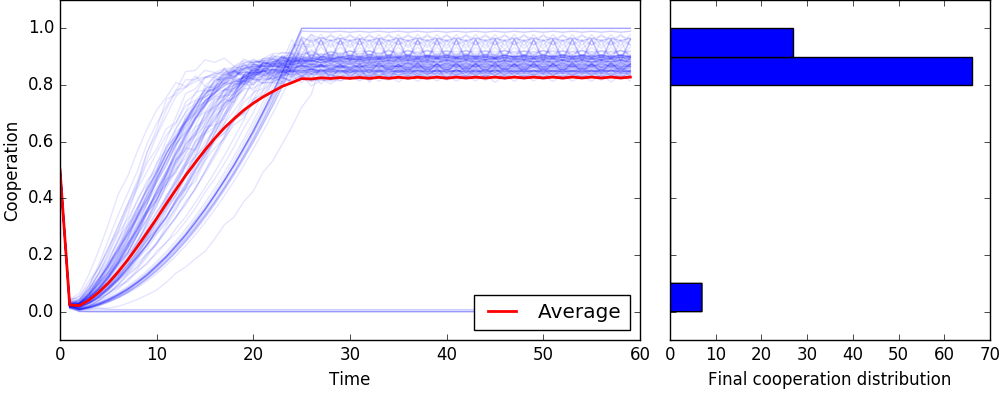
\includegraphics[width=0.7\textwidth]{./fig/n50.png}
	\caption{Cooperation levels of 100 runs along with their average
	on a 50x50 grid}
	\label{n50}
\end{figure}
Note that a stationary state does not necessarily mean that all simulations
have stopped moving. In fact, most of them reach a periodic equilibrium (as
can be seen with the sawteeth patterns appearing on figure \ref{n50}.\\

Most simulations reach a cooperation level between 80\% and 90\%. However, some
runs reach a total cooperation level while some dive very quickly to zero
cooperation.\\

Understanding the dynamics of this simulation starts by looking at figure
\ref{50viz}. When $t=5$, we clearly see clusters of cooperators (in magenta)
that expand until they meet other clusters (see when $t=10$). It makes sense
that these clusters expand because a defector right next to a single cluster
of cooperators will get a maximum payoff of $3T=30$ whereas a cooperator on 
the border of a cluster will get a payoff of $5R=35$; so the defector will
change his mind. This of course changes when two clusters meet : the defectors
stuck between two clusters will be able to take advantage of both clusters so
small trenches of defectors will remain and possibly oscillate as cooperators
want to take advantage of their cooperating neighbours.\\

A question remains: why do some runs delve to zero cooperation? This is
explained by the fact that the conditions for having a cluster are very harsh.
Indeed, in the first steps, most cooperators get wiped out unless they already
form a cluster large enough so that a core group of cooperators keeps
cooperating. A good example of this is the cluster that starts around the
coordinates (8,21).\\

\begin{figure}[H]
	\centering
	\subfloat[][$t=0$]{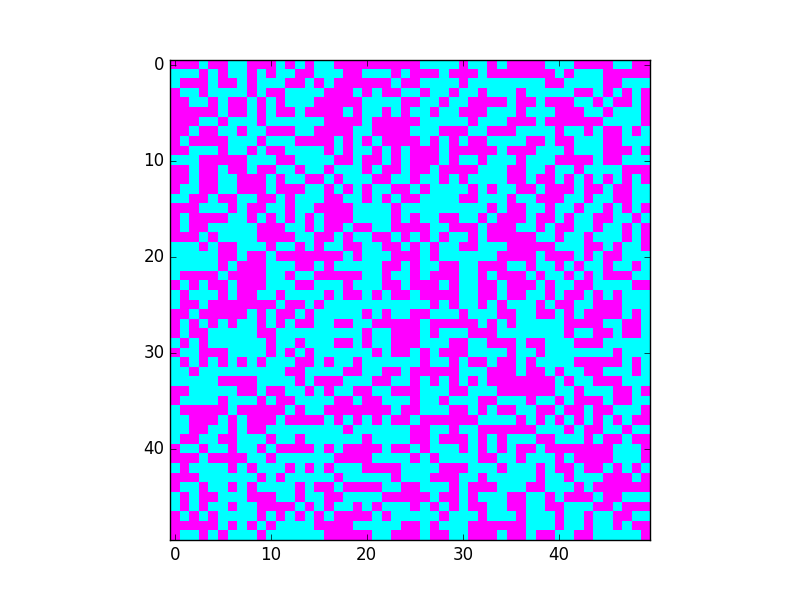
\includegraphics[width=.3\textwidth]{./fig/s0.png}}
	\subfloat[][$t=1$]{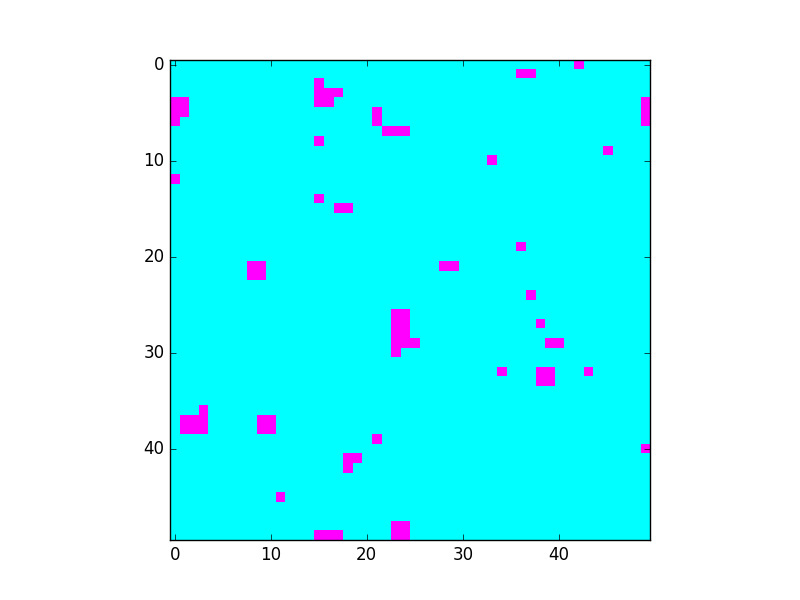
\includegraphics[width=.3\textwidth]{./fig/s1.png}}
	\subfloat[][$t=5$]{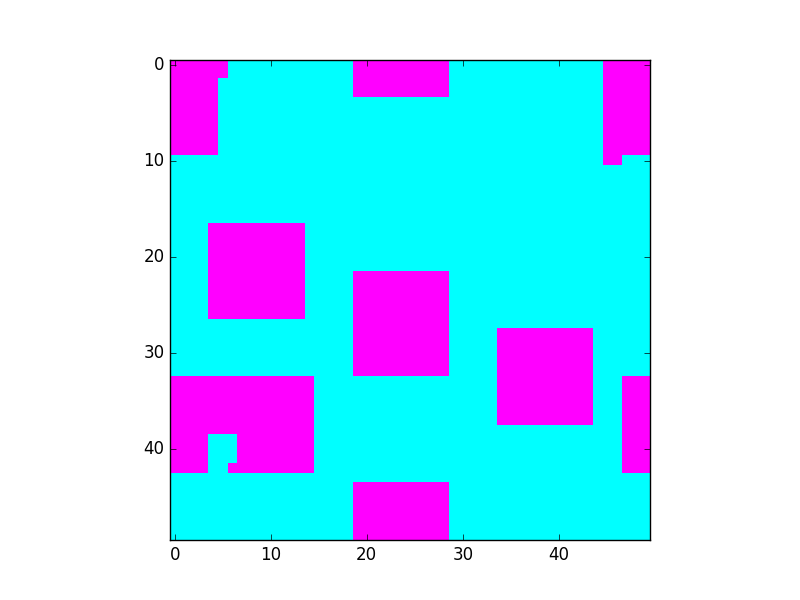
\includegraphics[width=.3\textwidth]{./fig/s5.png}}
	\\
	\subfloat[][$t=10$]{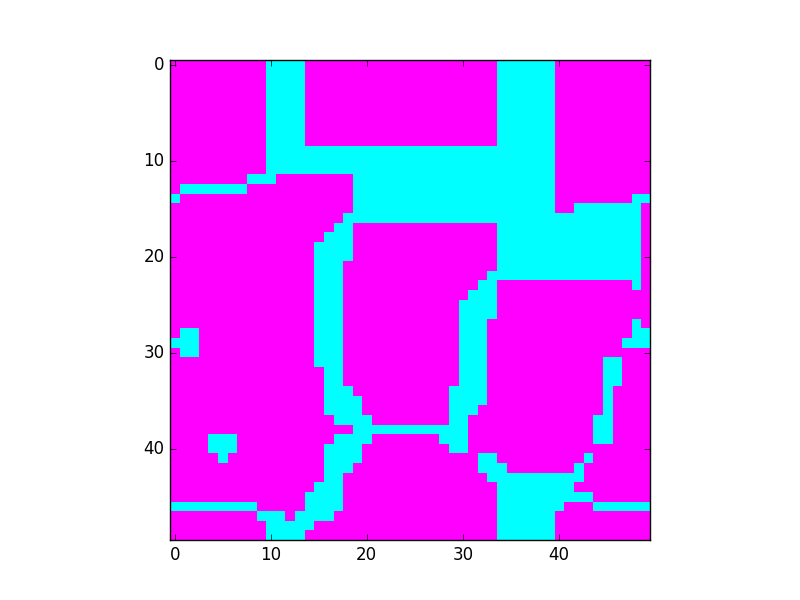
\includegraphics[width=.3\textwidth]{./fig/s10.png}}
	\subfloat[][$t=20$]{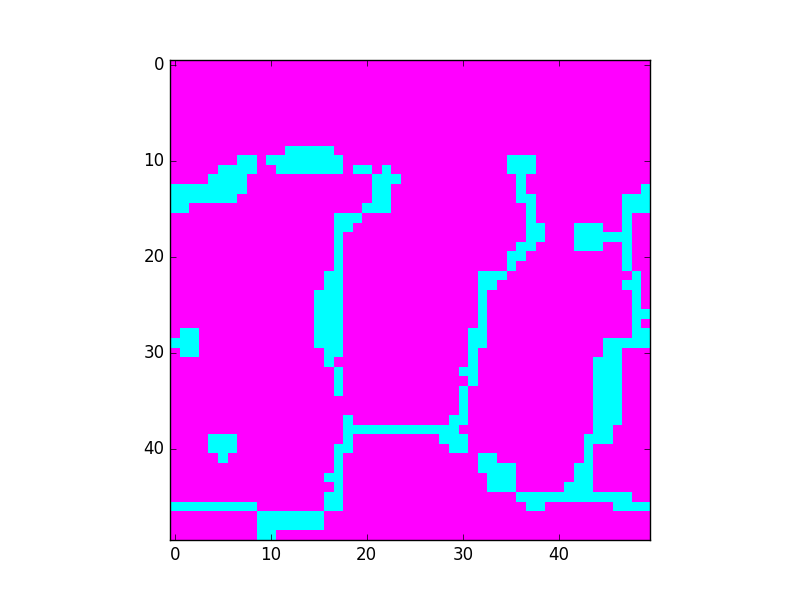
\includegraphics[width=.3\textwidth]{./fig/s20.png}}
	\subfloat[][$t=50$]{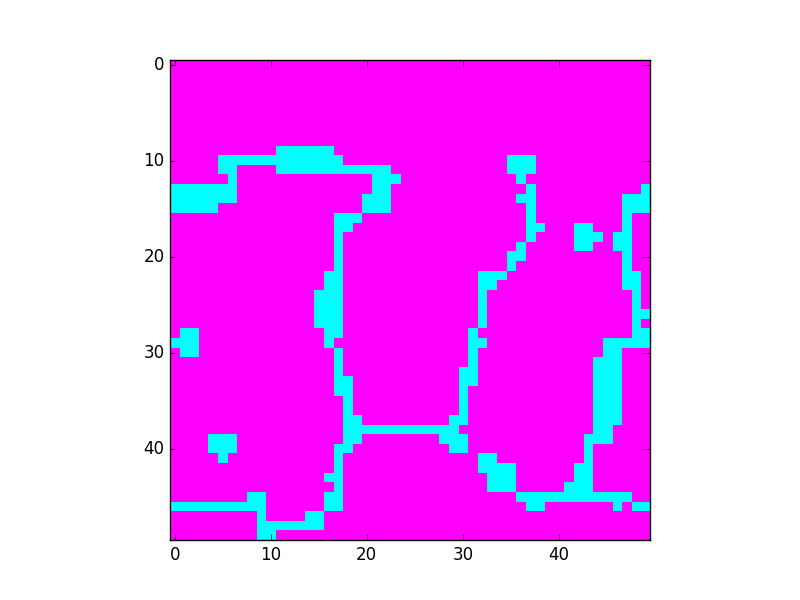
\includegraphics[width=.3\textwidth]{./fig/s50.png}}
	\caption{Evolution of one run on a 50x50 grid with defectors in cyan
	and cooperators in magenta}
	\label{50viz}
\end{figure}

This is exactly why, for a grid of size 4x4, the cooperation average is 
very close to zero : as clusters are fairly unlikely at the start and since
we don't have as many positions to start with (16 compared to 2500), the
probability of having a cluster is only 16/2500 times the one of a 50x50
grid. In fact, most runs of a 4x4 grid will end up falling to only defectors
after the second iteration (see figures \ref{4viz} and \ref{pr_m_convs}a).\\

\begin{figure}[H]
	\centering
	\subfloat[][$t=0$]{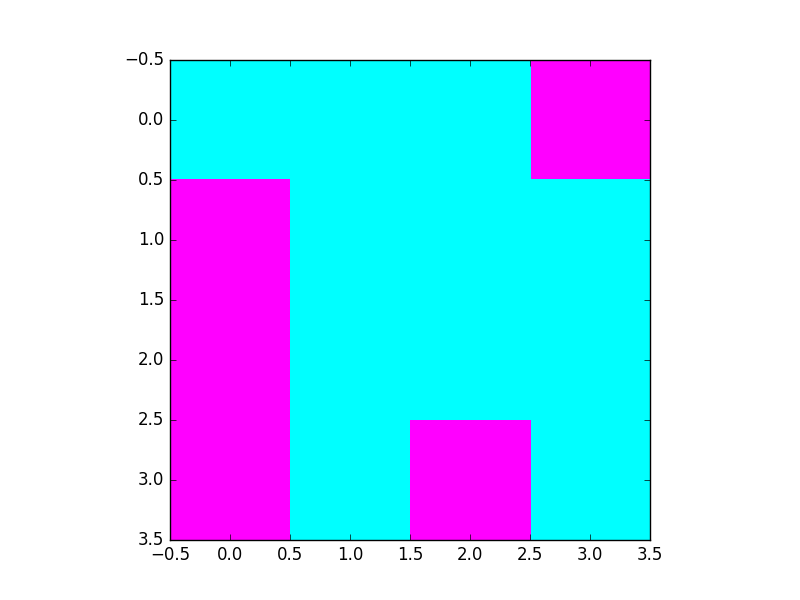
\includegraphics[width=.3\textwidth]{./fig/s4_0.png}}
	\subfloat[][$t=1$]{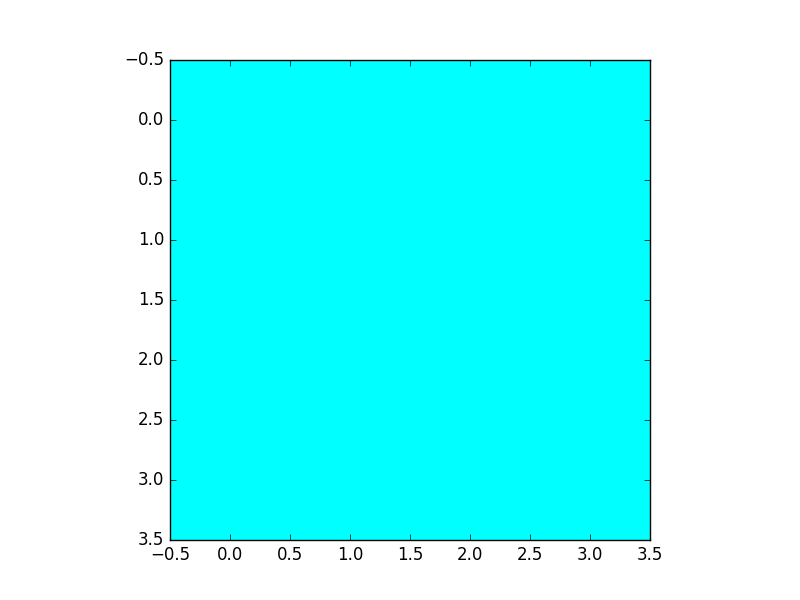
\includegraphics[width=.3\textwidth]{./fig/s4_1.png}}
	\caption{Evolution of one run on a 4x4 grid}
	\label{4viz}
\end{figure}

One thing worth noting, however, is that when the conditions are sufficient to
generate a cluster, the level of cooperation reached will always be around
80\%; only the proportion of simulations that reach it (instead of falling to
zero) changes. It is very clearly shown on figure \ref{pr_m_convs}).\\

We could say that the two modes of the bimodal distribution describing the 
final cooperation level never change; only the number of simulations belonging
to each mode changes, and the larger the grid is, the larger the number of 
simulations finishing with a high cooperation level will be.\\

Another observation, although trivial, would be to note that for smaller grids
that reach cooperation, the convergence is quicker as the clusters do not have
to grow for as much time as the larger grids before meeting either other
clusters or themselves because of the periodic boundary conditions.

\begin{figure}[H]
	\centering
	\subfloat[][4x4]{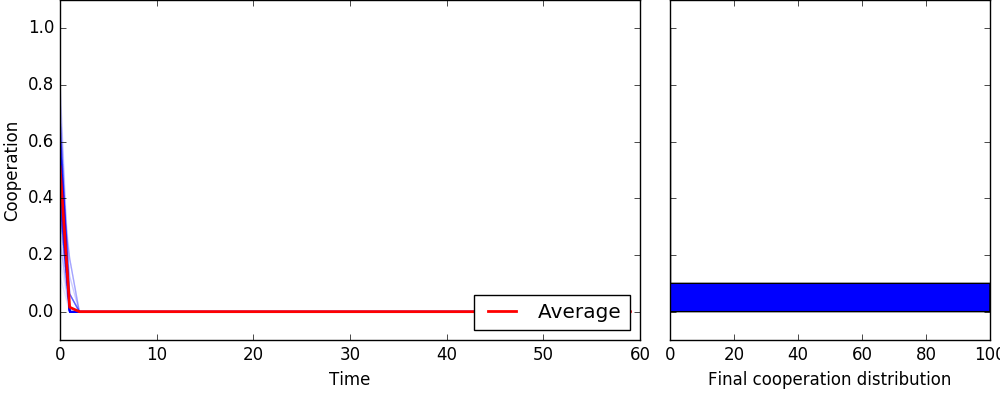
\includegraphics[width=.5\textwidth]{./fig/n4.png}}
	\subfloat[][8x8]{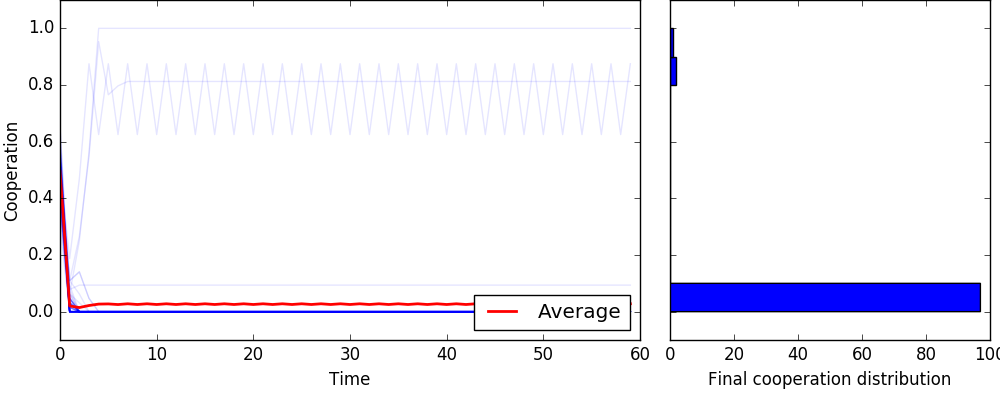
\includegraphics[width=.5\textwidth]{./fig/n8.png}}
	\\
	\subfloat[][12x12]{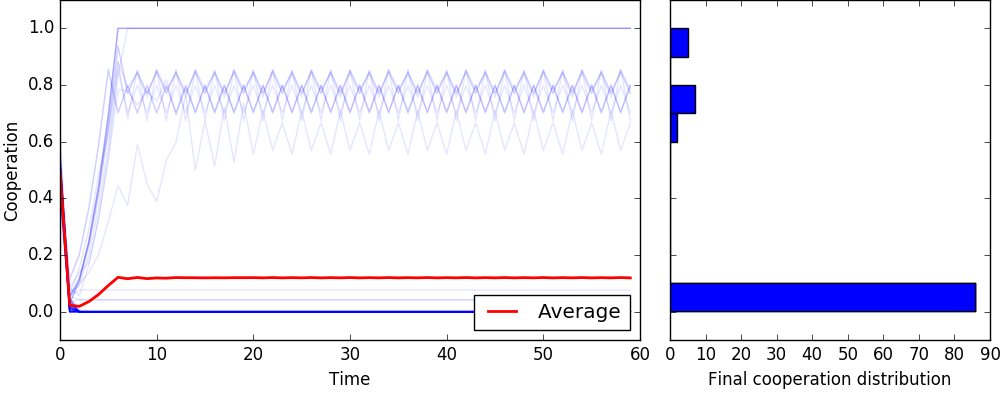
\includegraphics[width=.5\textwidth]{./fig/n12.png}}
	\subfloat[][20x20]{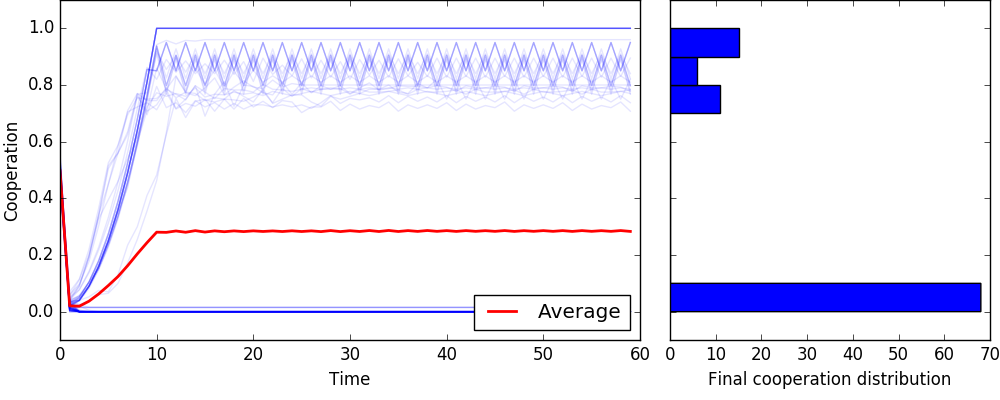
\includegraphics[width=.5\textwidth]{./fig/n20.png}}
	\caption{Variation of the convergence of runs with the grid size}
	\label{pr_m_convs}
\end{figure}

\subsection{Von Neumann neighbourhood}
Figure \ref{vn50} shows the convergence levels with the Von Neumann
neighbourhood. There are some striking differences with the Moore neighbourhood.
First, the average convergence level is much lower, at around 40\%, and second,
the runs do not seem to stabilise as much as with the Moore neighbourhood; 
their period seems to be much longer. Also, no run makes it to 100\% or 0\%
cooperation. They all stay very close to 40\% cooperation. 

\begin{figure}[H]
	\centering
	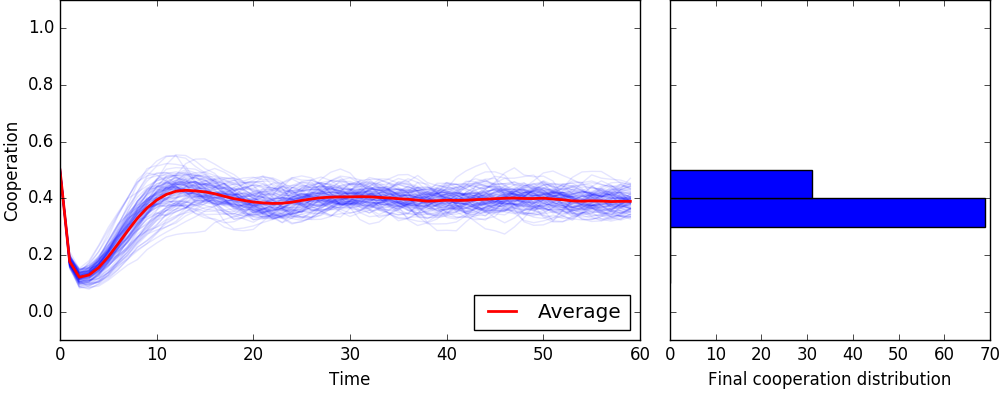
\includegraphics[width=0.7\textwidth]{./fig/vn_50.png}
	\caption{Cooperation levels of 100 runs along with their average
	on a 50x50 grid with the Von Neumann neighbourhood}
	\label{vn50}
\end{figure}

Let us try to understand why this is happening by looking at an example run
on figure \ref{vnviz}.

\begin{figure}[H]
	\centering
	\subfloat[][$t=0$]{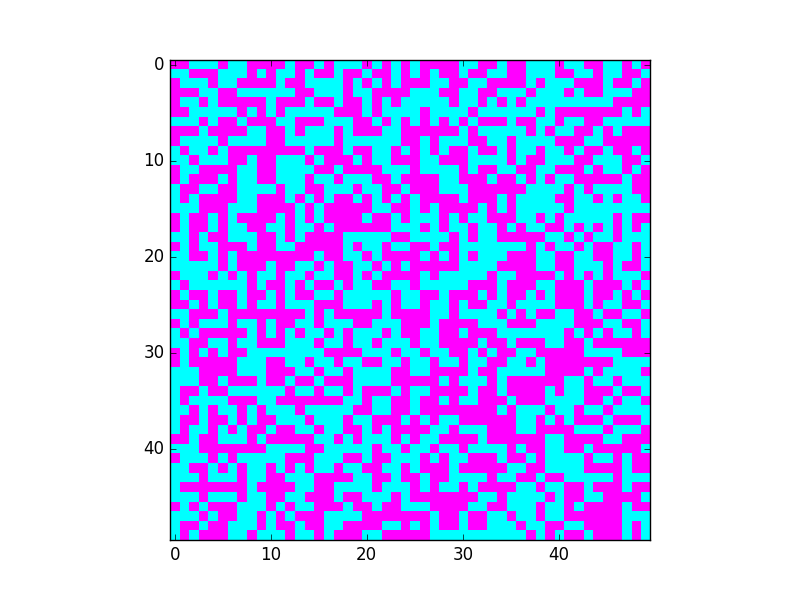
\includegraphics[width=.3\textwidth]{./fig/vn_s0.png}}
	\subfloat[][$t=1$]{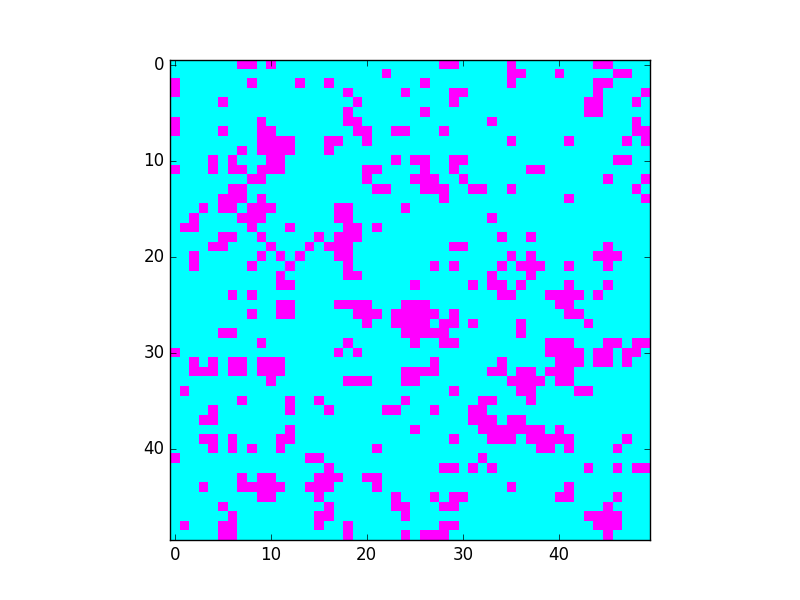
\includegraphics[width=.3\textwidth]{./fig/vn_s1.png}}
	\subfloat[][$t=5$]{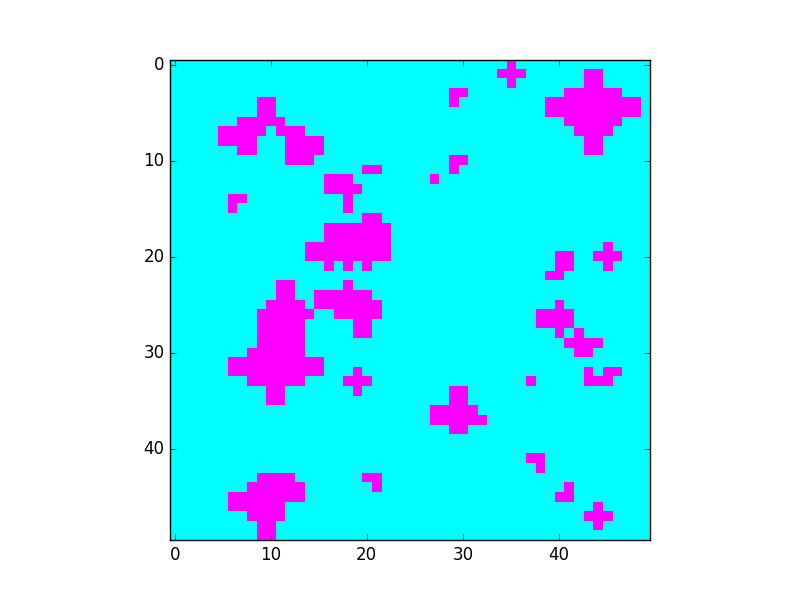
\includegraphics[width=.3\textwidth]{./fig/vn_s5.png}}
	\\
	\subfloat[][$t=10$]{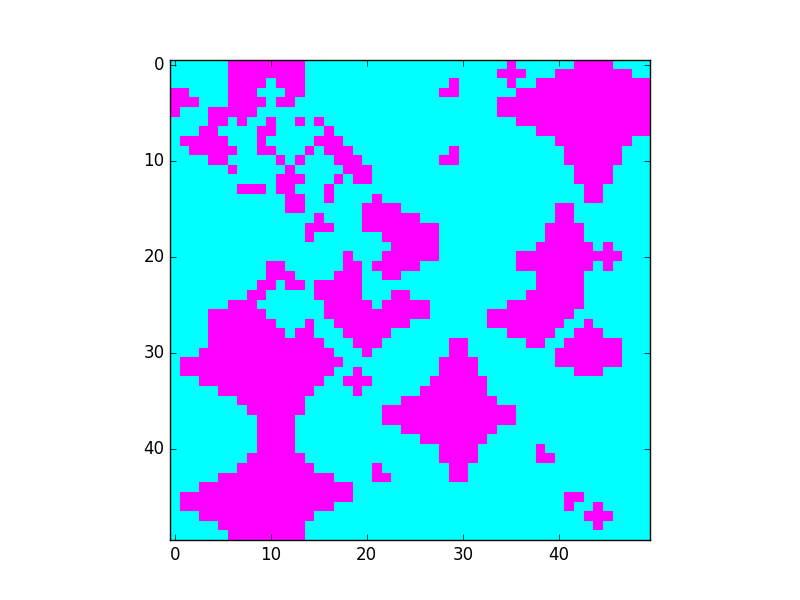
\includegraphics[width=.3\textwidth]{./fig/vn_s10.png}}
	\subfloat[][$t=20$]{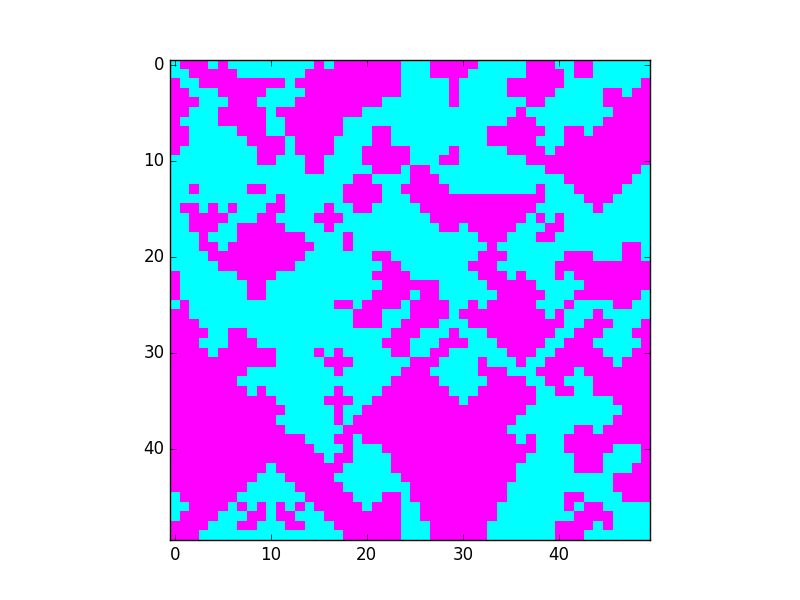
\includegraphics[width=.3\textwidth]{./fig/vn_s20.png}}
	\subfloat[][$t=50$]{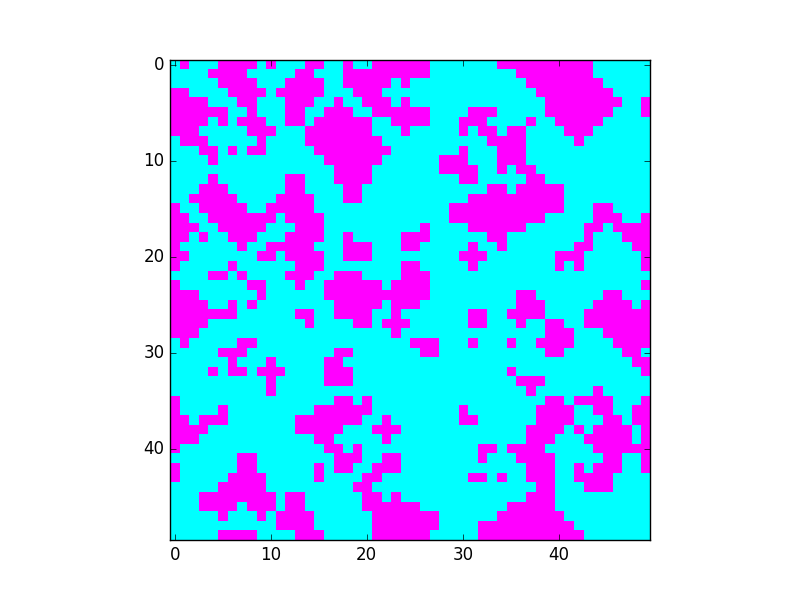
\includegraphics[width=.3\textwidth]{./fig/vn_s50.png}}
	\caption{Evolution of one run on a 50x50 grid with the Von Neumann
	Neighbourhood}
	\label{vnviz}
\end{figure}

A first noticeable difference is that the boundaries between cooperators and
defectors are now more diagonal rather than horizontal or vertical. In the 
case of the Von Neumann neighbourhood, once the original clusters have 
expanded, it becomes more interesting for the cooperators on the border of
a cluster near another one to become a defector, so the boundaries between
clusters will start growing again while clusters of cooperators will continue
expanding into defector-only regions, creating an endlessly moving pattern.


\end{document}
